\documentclass{article}
\usepackage[utf8]{inputenc}
\usepackage{amssymb}
\usepackage{natbib}
\bibliographystyle{plain}
\usepackage[fleqn]{amsmath}
\usepackage{amsthm}
\newtheorem{theorem}{Theorem}
\usepackage{graphicx}

\title{approximation-pattern}
\author{nguyenngockhanh.pbc }
\date{March 2021}

\begin{document}

\maketitle

Consider the problem of minimizing a function $f: D \to \mathbb{R}$

In many scenarios, it is hard to find an optimal, or it is even also hard to compute the value of $f$.
The method below was inspired from the work of Isaac Vandermeulen, Roderich Groß, Andreas Kolling~\cite{vandermeulen2019balanced}.

For a domain $X \subseteq D$ of the minimization problem,  let $f_1: X \to \mathbb{R}$ be the proxy function such that
\[
    (1): f(x) = c(f_1(x)) + v(x) \text{ } \forall x \in x
\]

Where $c$ is a monotonically increasing function and $v: X \to \mathbb{R}$ is function on $X$.

Let $x^*$ and $x^*_1$ be the optimal values for $f$ and $f_1$ in the domain $X \subseteq D$.
Let $t_{\max} = \max_{x \in X} v(x)$ and $t_{\min} = \min_{x \in X} v(x)$ be the maximum value and minimum value of $v$ over the domain $X$.  \footnote{Here, we used the maximum value and minimum value for $v$ since in the original work \cite{vandermeulen2019balanced}, the authors did not make it clear why $x^*$ and $x^*_1$ are independent from $v$ and further more, their proof does not make a clear statement on the feasibility of the method to any problem but rather most problems.}

\begin{figure}[h!]
\centering
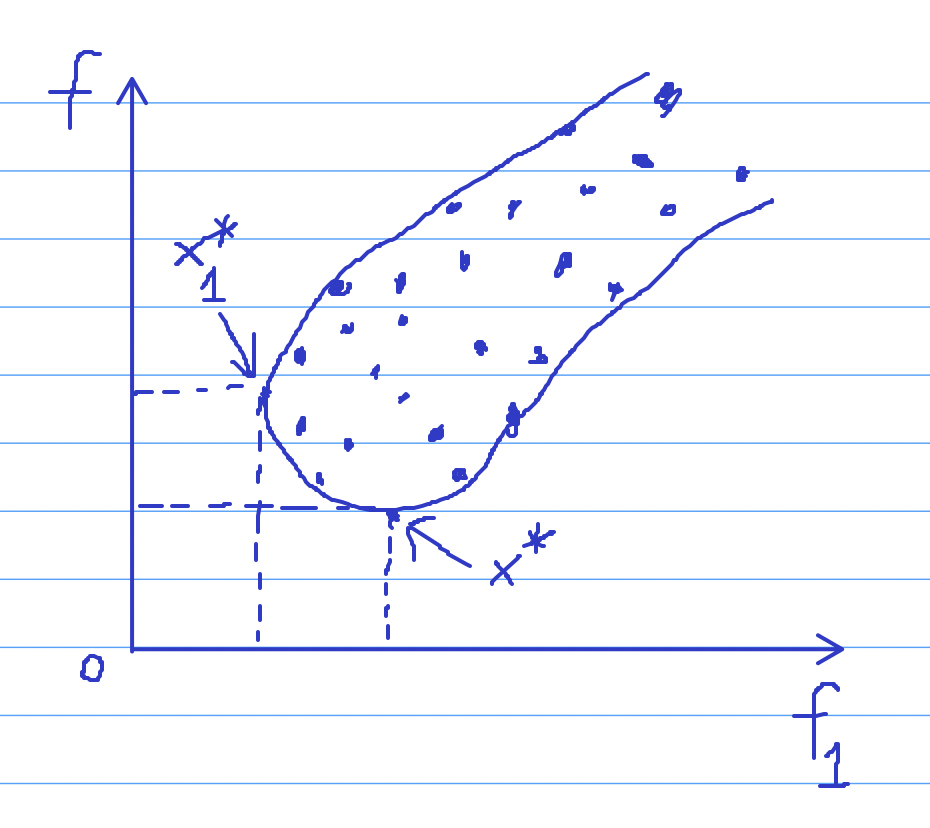
\includegraphics[width=0.8\textwidth]{f1_approximation.png}
\caption{$f_1 approximation$}
\label{fig:f1_approximation}
\end{figure}


Consider 3 inequalities:
\begin{gather*}
    (A): f(x^*_1) \leq f(x^*) + t_{\max} - t_{\min}\\
    (B): f(x^*_1) \leq c(f_1(x^*_1)) + t_{\max}\\
    (C): f(x^*) \geq c(f_1(x^*)) + t_{\min}\\
\end{gather*}

We have $f(x^*) \leq f(x^*_1)$ and $f_1(x^*_1) \leq f_1(x^*)$.
Since $c$ is a monotonically increasing function, so that $c(f_1(x^*_1)) \leq c(f_1(x^*))$.


By definition of $t_{\max}$, $(B)$ holds,
\[
    f(x^*_1) \leq c(f_1(x^*_1)) + t_{\max} \leq c(f_1(x^*)) + t_{\max}
\]

By definition of $t_{\min}$, $(C)$ holds,
\[
    f(x^*) \geq c(f_1(x^*)) + t_{\min} = (c(f_1(x^*)) + t_{\max}) - (t_{\max} - t_{\min})
\]

Hence,
\[
    (A): f(x^*_1) \leq f(x^*) + (t_{\max} - t_{\min})
\]

By choosing an appropriate proxy function $f_1$, we can approximate the solution of $f$.

In the derivation, we have set $t_{\max}$ and $t_{\min}$ be the maximum and minimum value of $v$ in the domain of $X$.
However, the bound can be even better if we have some methods to approximate the maximum and minimum value of $v$ in a subset of $X$ that contains both $x^*$ and $x^*_1$
\bibliography{references}





\end{document}
